\documentclass[conference]{IEEEtran}
\IEEEoverridecommandlockouts

\usepackage{cite}
\usepackage{amsmath,amssymb,amsfonts}
\usepackage{graphicx}
\usepackage{booktabs}
\usepackage{tikz}
\usetikzlibrary{arrows.meta,positioning,calc,fit}
\usepackage{textcomp}
\usepackage{xcolor}
\usepackage{microtype}
\usepackage[hidelinks]{hyperref}

\def\BibTeX{{\rm B\kern-.05em{\sc i\kern-.025em b}\kern-.08em
    T\kern-.1667em\lower.7ex\hbox{E}\kern-.125em X}}

\newcommand{\todoauthor}[1]{\textcolor{red}{#1}}

\begin{document}

\title{Connectome-Constrained Digital Twins of Longitudinal Neurodegeneration on OASIS-2: Network Diffusion, Graph Neural ODE and Generative Forecasting with an Interactive 3D Simulator}

\author{
\IEEEauthorblockN{Krish Sarkar}
\IEEEauthorblockA{\textit{Computer Science and Business Systems}\\
\textit{Mukesh Patel School of Technology}\\
\textit{Management and Engineering}\\
Mumbai, India\\
krish.sarkar62@nmims.in}
\and
\IEEEauthorblockN{Mithil Save}
\IEEEauthorblockA{\textit{Computer Science and Business Systems}\\
\textit{Mukesh Patel School of Technology}\\
\textit{Management and Engineering}\\
Mumbai, India\\
mithil.save81@nmims.in}
\and
\IEEEauthorblockN{Sofia Francis}
\IEEEauthorblockA{\textit{Computer Engineering}\\
\textit{Mukesh Patel School of Technology}\\
\textit{Management and Engineering}\\
Mumbai, India\\
sofia.francis@nmims.edu}
}

\maketitle

\begin{abstract}
Forecasting where in the brain neurodegeneration is present and where it will spread next is central to personalised dementia care. We present a regional \emph{digital twin} pipeline built on the longitudinal OASIS-2 cohort (150 older adults, 373 MRI sessions). Each subject is represented on a 56-region graph; regional volumes are converted to age-normalised atrophy scores (W-scores) and propagated over a connectome Laplacian. We implement four forecasters on this representation: the classical linear Network Diffusion Model (NDM) as a baseline, and three learned models designed for irregularly spaced visits---a spatio-temporal Graph Neural ODE (ST-GNN-ODE), a physics-regularised Network-Diffusion VAE (ND-VAE), and a temporally conditioned diffusion model (TADM). Regional atrophy is mapped to eleven cognitive-domain deficit scores through a region-to-domain weight map, and everything is exposed through an interactive 3D simulator with a time slider, region-level focus and an explainability panel. We report two simulator case studies, a nondemented control and a subject with CDR~0.5, and analyse them in detail. The analysis also exposes a limitation: large fitted diffusivities on our surrogate connectome drive the NDM state toward spatial uniformity, which is consistent with the identical domain scores observed at year~3.3. We do not report predictive benchmarks; the contribution is the framework, its honest scoping and a qualitative demonstration.
\end{abstract}

\begin{IEEEkeywords}
digital twin, Alzheimer's disease, network diffusion model, neural ODE, graph neural network, longitudinal MRI, OASIS-2
\end{IEEEkeywords}

%=====================================================================
\section{Introduction}
Neurodegenerative disease advances along anatomically structured paths: atrophy typically appears first in medial temporal regions and spreads through connected cortex. Two practical questions follow for any individual patient: \emph{which regions are affected now}, and \emph{which regions are likely to be affected next}? Answering them from routine structural MRI would support monitoring and counselling without requiring PET or fluid biomarkers.

The Network Diffusion Model (NDM) of Raj et~al.~\cite{raj2012ndm,raj2015ndm} explains spread as linear diffusion of pathology over the structural connectome, $x(t)=e^{-\beta Lt}x(0)$. It is compact and interpretable, but it is linear, has a single scalar rate, and cannot express region-specific dynamics. Longitudinal cohorts such as OASIS-2~\cite{marcus2010oasis} add a further difficulty: follow-up intervals are irregular (a few months to over seven years), which discrete-time recurrent models handle poorly.

This paper builds a pipeline that treats the NDM as a physics-based baseline and adds three learned continuous-time forecasters on the same 56-region graph, then surfaces the results in an interactive 3D digital-twin simulator. Our contributions are:
\begin{enumerate}
\item An end-to-end OASIS-2 pipeline from segmentation to age-normalised regional atrophy scores, a connectome Laplacian, and a per-subject NDM fit (Sections~\ref{sec:data}--\ref{sec:methods}).
\item Implementations of ST-GNN-ODE, ND-VAE and TADM that share one dataset, one graph and one evaluation harness, with subject-level data splits.
\item A region-to-cognitive-domain deficit mapping that turns a regional atrophy vector into eleven domain scores.
\item A qualitative analysis of two simulator case studies, including a diagnosis of an over-smoothing behaviour of the diffusion baseline (Section~\ref{sec:results}).
\end{enumerate}
We are explicit about scope. The connectome is a synthetic surrogate, predictive benchmarks are not yet reported, and the simulator is described only from its observable behaviour.

%=====================================================================
\section{Related Work}
\textbf{Network diffusion and spread models.} Raj et~al.\ introduced the NDM for dementia~\cite{raj2012ndm} and showed that, with a healthy reference connectome, it predicts longitudinal atrophy and metabolism patterns in Alzheimer's disease~\cite{raj2015ndm}. We follow this ``reference connectome'' practice because OASIS-2 contains no diffusion MRI.

\textbf{Continuous-time and graph models.} Neural ODEs~\cite{chen2018neuralode} define hidden-state dynamics by a learned vector field and integrate to arbitrary times; latent-ODE variants target irregularly sampled series~\cite{rubanova2019latentode}. Graph attention~\cite{velickovic2018gat} and graph convolution~\cite{kipf2017gcn} supply the spatial operator. Physics-informed learning~\cite{raissi2019pinn} motivates penalising deviation from a governing equation, which we apply to the diffusion law.

\textbf{Generative forecasting.} Variational autoencoders~\cite{kingma2014vae} give a probabilistic latent trajectory code. Denoising diffusion models~\cite{ho2020ddpm}, their fast implicit sampler~\cite{song2021ddim}, the cosine noise schedule~\cite{nichol2021improved} and feature-wise conditioning~\cite{perez2018film} underlie our conditional generator.

\textbf{Digital twins and evaluation practice.} Virtual brain twins personalise whole-brain network models to individuals~\cite{wang2024vbt}. For MRI classification, slice-level splitting leaks information and inflates accuracy; on OASIS the reported inflation is about 30 percentage points~\cite{yagis2021leakage}, and reproducible evaluation protocols are discussed in~\cite{wen2020cnn}. We therefore split strictly by subject. Attribution by integrated gradients~\cite{sundararajan2017ig} is the explainability method referenced by our simulator.

%=====================================================================
\section{Data and Preprocessing}\label{sec:data}
\subsection{Cohort}
OASIS-2 contains longitudinal T1-weighted MRI from 150 subjects aged 60--96 acquired on one scanner~\cite{marcus2010oasis}. The demographics file in our repository lists 373 sessions: 94 subjects have two visits, 43 have three, 9 have four and 4 have five (Fig.~\ref{fig:cohort}). At baseline 72 subjects are nondemented, 64 demented and 14 ``converted'' (nondemented at entry, demented later); 88 are female and 62 male. Baseline age is $75.4\pm7.5$ years and baseline MMSE $27.6\pm3.0$. Across all sessions the Clinical Dementia Rating (CDR) is 0 in 206, 0.5 in 123, 1 in 41 and 2 in 3. The longest follow-up from baseline is 2639 days (7.2 years). Only these tabular fields are used directly by the learned models; regional features come from the segmentation step below.

\begin{figure*}[t]
\centering
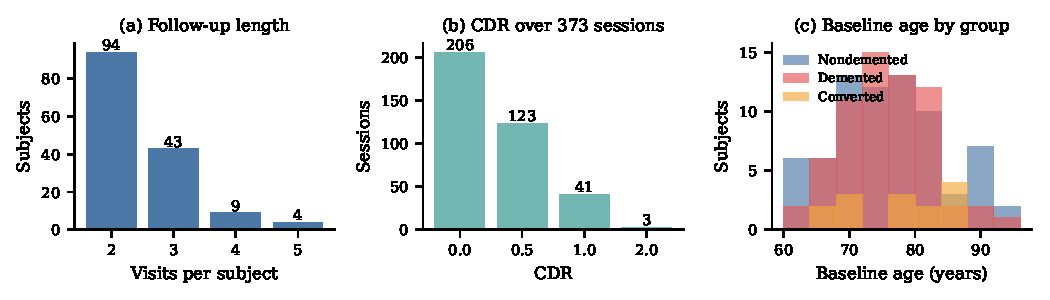
\includegraphics[width=\textwidth]{figures/fig_cohort.pdf}
\caption{OASIS-2 cohort as used here (from the demographics file). (a) Number of visits per subject. (b) CDR distribution over all 373 sessions. (c) Baseline age by baseline group.}
\label{fig:cohort}
\end{figure*}

\begin{figure*}[t]
\centering
\resizebox{0.98\textwidth}{!}{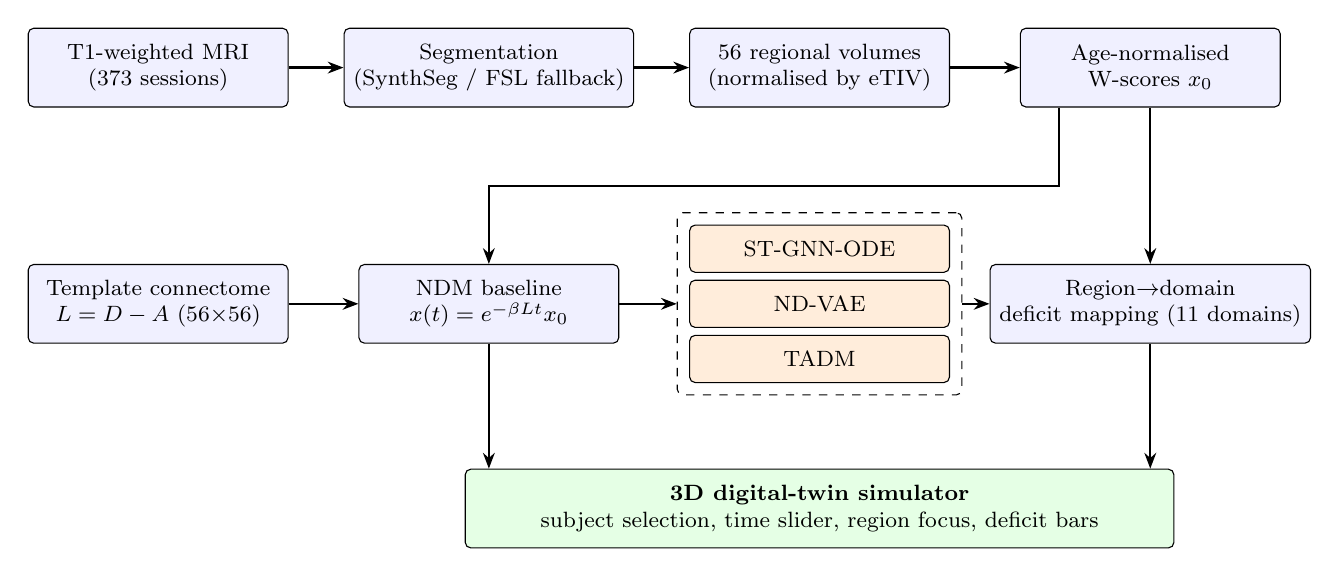
\begin{tikzpicture}[
  font=\footnotesize,
  box/.style={draw, rounded corners=2pt, minimum height=10mm, minimum width=33mm, align=center, fill=blue!6},
  mdl/.style={draw, rounded corners=2pt, minimum height=6mm, minimum width=33mm, align=center, fill=orange!14},
  fin/.style={draw, rounded corners=2pt, minimum height=10mm, minimum width=33mm, align=center, fill=green!10},
  arr/.style={-{Stealth[length=2mm]}, thick}
]
% Row 1
\node[box] (mri) at (0,0) {T1-weighted MRI\\(373 sessions)};
\node[box] (seg) at (4.2,0) {Segmentation\\(SynthSeg / FSL fallback)};
\node[box] (vol) at (8.4,0) {56 regional volumes\\(normalised by eTIV)};
\node[box] (w)   at (12.6,0) {Age-normalised\\W-scores $x_0$};
\draw[arr] (mri) -- (seg);
\draw[arr] (seg) -- (vol);
\draw[arr] (vol) -- (w);

% Row 2
\node[box] (conn) at (0,-3.0) {Template connectome\\$L=D-A$ (56$\times$56)};
\node[box] (ndm)  at (4.2,-3.0) {NDM baseline\\$x(t)=e^{-\beta Lt}x_0$};
\node[mdl] (m1) at (8.4,-2.3) {ST-GNN-ODE};
\node[mdl] (m2) at (8.4,-3.0) {ND-VAE};
\node[mdl] (m3) at (8.4,-3.7) {TADM};
\node[box] (map) at (12.6,-3.0) {Region$\to$domain\\deficit mapping (11 domains)};
\draw[arr] (conn) -- (ndm);

\node[draw, dashed, rounded corners=2pt, fit=(m1)(m2)(m3), inner sep=1.5mm] (fc) {};
\draw[arr] (ndm) -- (fc.west);
\draw[arr] (fc.east) -- (map);
\draw[arr] (w.south) -- (map.north);
\draw[arr] (w.south west) ++(5mm,0) -- ++(0,-1.0) -| (ndm.north);

% Row 3
\node[fin, minimum width=90mm] (sim) at (8.4,-5.6) {\textbf{3D digital-twin simulator}\\subject selection, time slider, region focus, deficit bars};
\draw[arr] (map.south) -- (map.south |- sim.north);
\draw[arr] (ndm.south) -- (ndm.south |- sim.north);
\end{tikzpicture}
}
\caption{Pipeline overview. Segmentation yields regional volumes that are normalised to W-scores; the template connectome supplies the Laplacian used by the NDM baseline and the graph operators of the learned forecasters; predicted regional atrophy is mapped to cognitive-domain deficits and displayed in the 3D simulator.}
\label{fig:pipeline}
\end{figure*}

\subsection{Regional parcellation and W-scores}
The pipeline defines $N=56$ regions named in the Desikan--Killiany convention~\cite{desikan2006atlas}: 34 left-hemisphere cortical labels, 10 subcortical structures (bilateral hippocampus, amygdala, thalamus, caudate and putamen), and 12 right-hemisphere cortical labels. Regional volumes are produced by SynthSeg~\cite{billot2023synthseg} where it is installed, with a FSL-based fallback, and are normalised by estimated total intracranial volume (eTIV).

To remove normal ageing from the pathology signal we compute W-scores. For each region, a linear regression of normalised volume on age is fitted on sessions with CDR~$=0$; each session's residual is then standardised by the residual mean and standard deviation of that reference set, and the sign is flipped so that atrophy is positive. A W-score of $+1$ therefore means one standard deviation less tissue than expected for that age. The resulting vector $x\in\mathbb{R}^{56}$ is the node-feature channel of every model.

\subsection{Template connectome and Laplacian}
Regional spread is constrained by a $56\times56$ template adjacency $A$. The shipped template is a \emph{synthetic surrogate}: it is generated with a fixed seed from exponentially distributed weights, thresholded at the 80th percentile, with additional edge weight (+0.5) among hippocampus, entorhinal and parahippocampal regions to encode the known medial-temporal vulnerability. The resulting matrix is symmetric with 20.8\% non-zero entries. The Laplacian is $L=D-A$ with $D$ the weighted degree matrix; its eigenvalues range from $0$ to $15.9$, with the smallest non-zero value $\lambda_2=2.58$ (Fig.~\ref{fig:spectrum}a). A real reference connectome (for example the Budapest or HCP atlases) should replace this surrogate; see Section~\ref{sec:limits}.

\begin{figure*}[t]
\centering
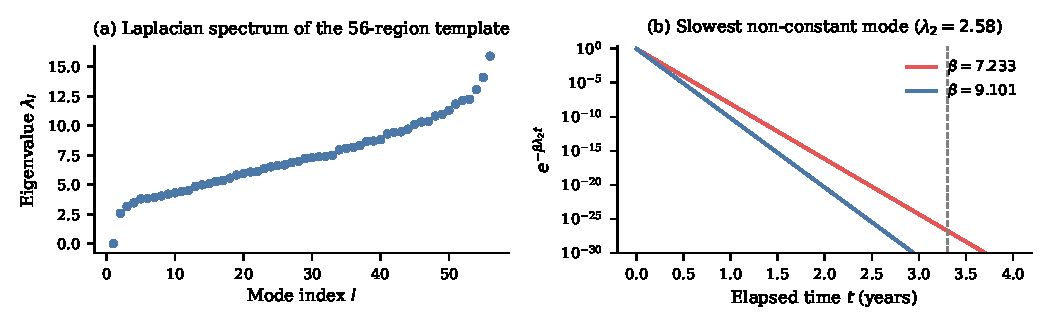
\includegraphics[width=0.85\textwidth]{figures/fig_ndm_spectrum.pdf}
\caption{Spectral view of the template connectome. (a) Laplacian eigenvalues of the 56-region surrogate. (b) Attenuation $e^{-\beta\lambda_2 t}$ of the slowest non-constant diffusion mode for the two diffusivities shown in the simulator screenshots; the dashed line marks $t=3.3$ years. Note the logarithmic axis.}
\label{fig:spectrum}
\end{figure*}

%=====================================================================
\section{Methods}\label{sec:methods}
\subsection{NDM baseline}
Pathology spreads as $\dot x=-\beta Lx$, with closed form $x(t)=e^{-\beta Lt}x(0)$. With the eigendecomposition $L=V\Lambda V^\top$ computed once,
\begin{equation}
x(t)=V\,\mathrm{diag}\!\left(e^{-\beta\lambda_i t}\right)V^\top x(0).
\end{equation}
For each subject the scalar $\beta$ is fitted by bounded one-dimensional minimisation of the squared error between predicted and observed W-scores at the first follow-up, with $\beta\in[0.001,10]$ and $t$ in years. Validation uses subjects with at least three visits: $\beta$ fitted on visit~2 is used to predict visit~3, and Pearson correlation and MSE are computed over regions.

\subsection{Learned forecasters}
All three models take the baseline state $X(t_0)\in\mathbb{R}^{N\times1}$, static covariates $c\in\mathbb{R}^6$ (age, sex, education, SES, eTIV, ASF, each scaled), the normalised adjacency $\hat A=\tilde D^{-1/2}(A+I)\tilde D^{-1/2}$ with $\tilde D$ the degree matrix of $A+I$, and irregular visit times in years from baseline (Fig.~\ref{fig:models}). Clinical heads predict MMSE (scaled to $[0,1]$) and a four-class CDR stage (0, 0.5, 1, 2).

\begin{figure*}[t]
\centering
\resizebox{0.95\textwidth}{!}{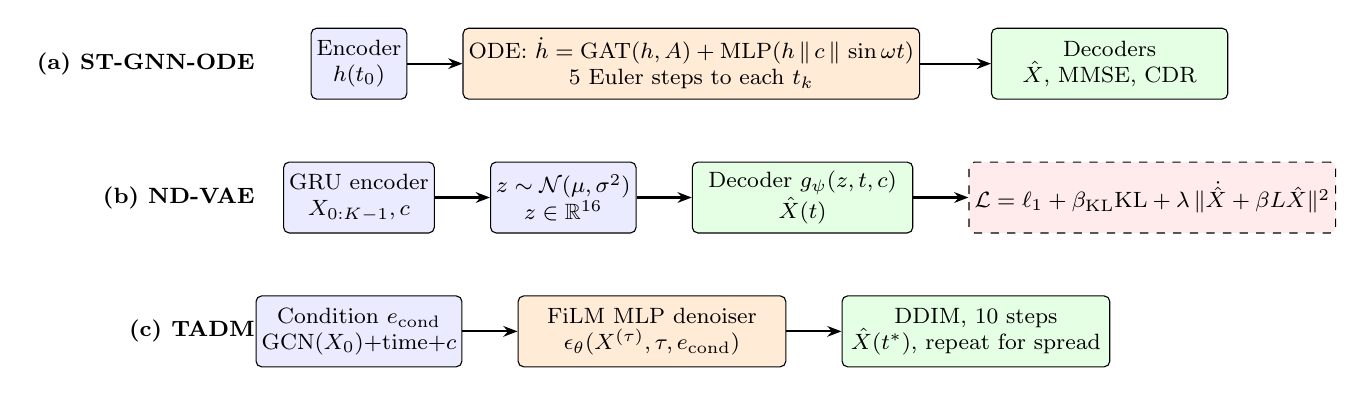
\begin{tikzpicture}[
  font=\footnotesize,
  n/.style={draw, rounded corners=2pt, minimum height=9mm, align=center, inner sep=2pt},
  enc/.style={n, fill=blue!8},
  core/.style={n, fill=orange!16},
  dec/.style={n, fill=green!10},
  loss/.style={n, fill=red!8, dashed},
  arr/.style={-{Stealth[length=1.8mm]}, thick},
  lab/.style={font=\bfseries\footnotesize, anchor=east}
]
% Row 1: ST-GNN-ODE
\node[lab] at (0,0) {(a) ST-GNN-ODE};
\node[enc] (a1) at (1.2,0) {Encoder\\$h(t_0)$};
\node[core, right=7mm of a1, minimum width=50mm] (a2) {ODE: $\dot h=\mathrm{GAT}(h,A)+\mathrm{MLP}(h\,\|\,c\,\|\,\sin\omega t)$\\5 Euler steps to each $t_k$};
\node[dec, right=9mm of a2, minimum width=30mm] (a3) {Decoders\\$\hat X$, MMSE, CDR};
\draw[arr] (a1) -- (a2); \draw[arr] (a2) -- (a3);

% Row 2: ND-VAE
\node[lab] at (0,-1.7) {(b) ND-VAE};
\node[enc] (b1) at (1.2,-1.7) {GRU encoder\\$X_{0:K-1},c$};
\node[enc, right=7mm of b1] (b2) {$z\sim\mathcal{N}(\mu,\sigma^2)$\\$z\in\mathbb{R}^{16}$};
\node[dec, right=7mm of b2, minimum width=28mm] (b3) {Decoder $g_\psi(z,t,c)$\\$\hat X(t)$};
\node[loss, right=7mm of b3, minimum width=40mm] (b4) {$\mathcal{L}=\ell_1+\beta_{\mathrm{KL}}\mathrm{KL}+\lambda\,\|\dot{\hat X}+\beta L\hat X\|^2$};
\draw[arr] (b1) -- (b2); \draw[arr] (b2) -- (b3); \draw[arr] (b3) -- (b4);

% Row 3: TADM
\node[lab] at (0,-3.4) {(c) TADM};
\node[enc] (c1) at (1.2,-3.4) {Condition $e_{\mathrm{cond}}$\\GCN$(X_0)$+time+$c$};
\node[core, right=7mm of c1, minimum width=34mm] (c2) {FiLM MLP denoiser\\$\epsilon_\theta(X^{(\tau)},\tau,e_{\mathrm{cond}})$};
\node[dec, right=7mm of c2, minimum width=34mm] (c3) {DDIM, 10 steps\\$\hat X(t^*)$, repeat for spread};
\draw[arr] (c1) -- (c2); \draw[arr] (c2) -- (c3);
\end{tikzpicture}
}
\caption{The three learned forecasters as implemented. (a) A graph-attention vector field integrated continuously in time. (b) A GRU-encoded latent trajectory code with a diffusion-physics penalty. (c) A conditional denoising generator sampled with DDIM.}
\label{fig:models}
\end{figure*}

\subsubsection{ST-GNN-ODE}
An MLP encodes $[X(t_0)\,\|\,c]$ to $h(t_0)\in\mathbb{R}^{N\times32}$. The latent state follows
\begin{equation}
\frac{dh}{dt}=f_\theta(h,t)=\mathrm{MLP}\big(\mathrm{GAT}(h;\hat A)\,\|\,c\,\|\,\phi(t)\big),
\end{equation}
where $\mathrm{GAT}$ is a single-head graph attention layer~\cite{velickovic2018gat} masked by $\hat A$ and $\phi(t)$ is a 16-dimensional sinusoidal time embedding. The state is advanced to each visit time by five explicit Euler steps; the design allows an adaptive solver~\cite{chen2018neuralode} but the implementation uses fixed steps for speed. A linear head reconstructs $\hat X(t_k)$ and two small heads on the mean-pooled state predict MMSE and CDR. The loss is $\mathrm{MSE}(\hat X,X)+0.5\,\mathrm{MSE}_{\mathrm{MMSE}}+0.3\,\mathrm{CE}_{\mathrm{CDR}}$.

\subsubsection{ND-VAE}
A GRU reads the visit sequence $[X(t_k)\,\|\,c]$ and outputs $(\mu,\log\sigma^2)$ of a $16$-dimensional latent code $z$. A decoder maps $(z,t,c)\mapsto\hat X(t)$. The objective is
\begin{equation}
\begin{split}
\mathcal{L}={}&\|\hat X-X\|_1+\beta_{\mathrm{KL}}\,D_{\mathrm{KL}}+\lambda_{\mathrm{phys}}\,\Big\|\tfrac{d\hat X}{dt}+\beta_{\mathrm{d}}L\hat X\Big\|^2\\
&+0.5\,\mathrm{MSE}_{\mathrm{MMSE}}+0.3\,\mathrm{CE}_{\mathrm{CDR}},
\end{split}
\end{equation}
with $\beta_{\mathrm{KL}}$ annealed linearly to $0.1$ over 20 epochs, $\lambda_{\mathrm{phys}}=0.01$, a learnable diffusion coefficient $\beta_{\mathrm{d}}$ initialised at $0.1$, and the time derivative approximated by finite differences between consecutive visits. Here $L=I-\hat A$.

\subsubsection{TADM}
For each baseline--future pair, the target $X_k$ is noised with a cosine schedule~\cite{nichol2021improved} over $T=200$ steps. A conditioning vector $e_{\mathrm{cond}}$ concatenates a pooled graph-convolution~\cite{kipf2017gcn} embedding of $X(t_0)$, a sinusoidal embedding of $\Delta t_k$, and a covariate embedding, projected to 32 dimensions. An MLP denoiser with FiLM modulation~\cite{perez2018film} predicts the added noise, and training minimises $\|\epsilon-\epsilon_\theta(X_k^{(\tau)},\tau,e_{\mathrm{cond}})\|^2$~\cite{ho2020ddpm}. Sampling uses 10 DDIM steps~\cite{song2021ddim}; repeated sampling from different noise seeds yields a spread that serves as an uncertainty estimate.

\subsection{Training protocol and metrics}
Subjects with at least two visits are split by subject into 70/15/15\% train/validation/test sets (seed 42), so no subject's visits cross sets; this follows the leakage-aware practice of~\cite{yagis2021leakage}. Training uses AdamW (learning rate $10^{-3}$, weight decay $10^{-4}$), cosine learning-rate decay, gradient clipping at 1.0, batch size 8, and early stopping on validation loss (patience 10, 10 and 15; at most 50, 100 and 200 epochs for ST-GNN-ODE, ND-VAE and TADM). The evaluation harness reports atrophy RMSE, MAE and Pearson $r$, MMSE MAE, and CDR accuracy and macro-F1, alongside the NDM baseline. The numerical benchmark is outside the scope of this paper.

\subsection{Cognitive-domain deficit mapping}
A weight map $w_{r,d}\in[0,1]$ links regions to eleven domains (episodic memory, executive function, language, visuospatial, emotional regulation, attention, working memory, semantic memory, learning, object recognition, behavioural control). For example, left hippocampus carries weight 1.0 for episodic memory and 0.8 for learning, and the left rostral middle frontal gyrus carries 1.0 for executive function. The deficit of domain $d$ is the weight-averaged atrophy $s_d=\sum_r w_{r,d}x_r/\sum_r w_{r,d}$ over regions with non-zero weight. The implementation then rescales the eleven scores to $[0,1]$ by min--max normalisation within the subject whenever their range is non-zero. Scores are therefore \emph{relative within a subject}, not calibrated risks.

\subsection{Interactive 3D simulator}
The simulator is the user-facing layer of the twin. From its interface (Figs.~\ref{fig:sim1} and~\ref{fig:sim2}) it offers: (i) a subject selector showing clinical group, age/sex, baseline CDR and the subject's fitted NDM diffusivity $\beta$; (ii) camera presets (superior, anterior, left lateral, isometric) with toggles for connectome tracts and auto-rotation; (iii) a 3D view of 56 region nodes coloured by atrophy W-score on a scale from healthy ($\le0$) to severe ($\ge+3$); (iv) a ``timeline horizon'' slider with a Simulate/Pause control, annotated with the propagation law $e^{-\beta Lt}x_0$; and (v) a side panel with the focused region, its simulated atrophy in $\sigma$ units, the eleven domain deficit bars, and an explainability note. We describe only what is visible in the interface and do not make claims about its implementation.

%=====================================================================
\section{Results: Simulator Case Studies}\label{sec:results}
We analyse two simulator sessions, one per figure. All values quoted below are read from the screenshots. No predictive accuracy is claimed from them; they illustrate the twin's outputs and expose their behaviour.

\subsection{Case A: nondemented control at baseline}
Fig.~\ref{fig:sim1} shows subject OAS2\_0001 (nondemented, 87 years, male, baseline CDR 0.0, fitted $\beta=9.101$) at timeline year 0.0, before any propagation. The 3D view shows 56 nodes of visibly different colour: most are cyan to blue, indicating W-scores near or below the healthy end of the scale, and a few are green, indicating mildly elevated atrophy. The focused region is the left insula (a left-hemisphere cortical parcel) with simulated atrophy $+0.82\,\sigma$, associated with emotional regulation and interoception.

The domain panel is spatially heterogeneous: object recognition (73\%), emotional regulation (71\%), behavioural control (66\%), attention and semantic memory (both 61\%), episodic memory (55\%), working memory (48\%), learning and visuospatial (both 43\%), executive function (40\%) and language (35\%). The ordering is driven by which weighted regions currently carry the highest W-scores. Two cautions follow from Section~\ref{sec:methods}. First, because scores are min--max normalised within a subject, a figure such as 73\% denotes the subject's \emph{most} affected domain, not a 73\% clinical risk; this subject has CDR 0.0. Second, the end label ``Severe Pathology'' on the colour bar is the label of the scale's maximum, not a statement about this subject.

\begin{figure*}[t]
\centering
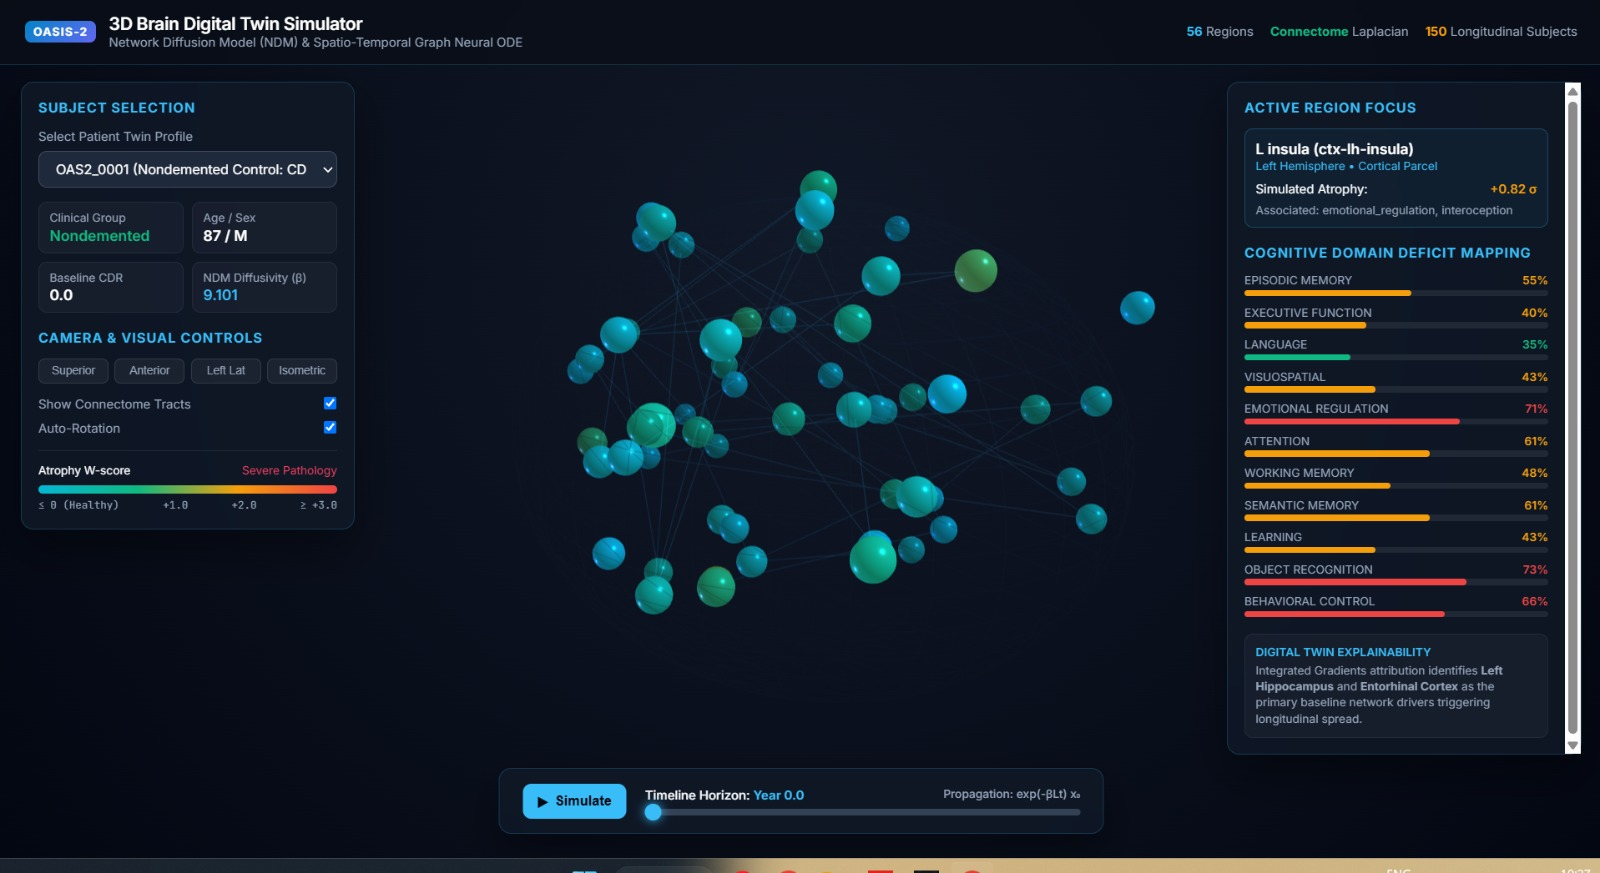
\includegraphics[width=0.96\textwidth]{figures/sim_cn_baseline.jpg}
\caption{Simulator view, Case A: subject OAS2\_0001 (nondemented, 87\,y, male, CDR 0.0, $\beta=9.101$) at year 0.0. Left: subject selection, camera controls and atrophy W-score legend. Centre: 56-region 3D view with connectome tracts. Right: focused region (left insula, $+0.82\sigma$), eleven cognitive-domain deficit bars and the explainability note. Bottom: Simulate control and timeline slider.}
\label{fig:sim1}
\end{figure*}

\subsection{Case B: subject with CDR 0.5 at year 3.3}
Fig.~\ref{fig:sim2} shows subject OAS2\_0002 (labelled demented, 75 years, male, baseline CDR 0.5, fitted $\beta=7.233$) while the simulation is running at timeline year 3.3 (the control reads ``Pause''). The focused region is the left hippocampus, a subcortical nucleus in the left hemisphere, with simulated atrophy $+0.94\,\sigma$ and associations with episodic memory and learning---the structures most closely tied to early Alzheimer's pathology. The explainability note names the left hippocampus and entorhinal cortex as the primary baseline network drivers of longitudinal spread, in line with the medial-temporal weighting built into the connectome.

Two features of this view need explanation. First, all eleven domain bars read an identical 94\%, and the 3D nodes are visually uniform in colour. Second, the displayed regional value ($+0.94\sigma$) equals the domain value, which is what one expects if every region has the same value. This pattern matches the spectral behaviour of the diffusion law. Under $e^{-\beta Lt}$ every non-constant mode decays, and the state converges to the regional mean of $x_0$. On the surrogate connectome the slowest such mode has $\lambda_2=2.58$ (Fig.~\ref{fig:spectrum}a), so with the fitted $\beta=7.233$ it is attenuated by a factor of about $9\times10^{-5}$ after only 0.5 years and about $2\times10^{-27}$ at 3.3 years (Fig.~\ref{fig:spectrum}b); for Case~A's $\beta=9.101$ the corresponding factors are $8\times10^{-6}$ and $2\times10^{-34}$. If the simulator measures $t$ in years as the $\beta$-fitting routine does, then by year 3.3 the NDM state has been flattened to its mean. Because the deficit map is a weighted \emph{average} of regional values, a constant state yields the same score in every domain, giving the uniform bars. We could not inspect the simulator code, so this is a consistent explanation rather than a confirmed one. Its implication is practical: at diffusivities of this size the baseline NDM carries almost no spatial information beyond the first few months, and the saturated view should not be read as clinical severity.

\begin{figure*}[t]
\centering
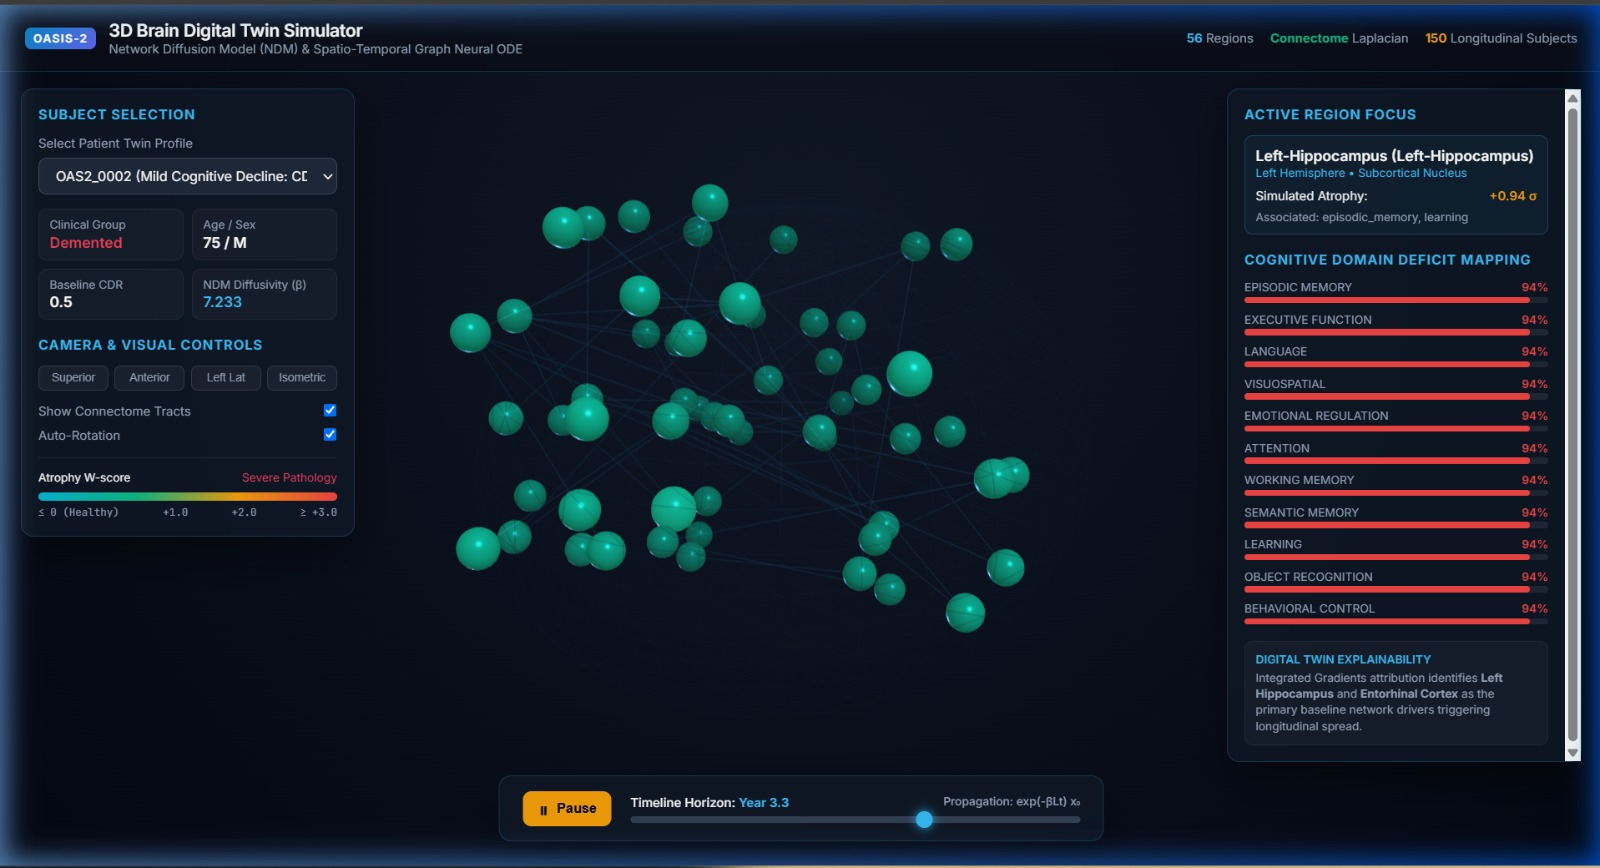
\includegraphics[width=0.96\textwidth]{figures/sim_demented_year3p3.jpg}
\caption{Simulator view, Case B: subject OAS2\_0002 (demented, 75\,y, male, CDR 0.5, $\beta=7.233$) at year 3.3 while simulating. The focused region is the left hippocampus ($+0.94\sigma$). All eleven domain deficit bars show 94\% and the nodes are uniformly coloured, consistent with a spatially homogeneous state.}
\label{fig:sim2}
\end{figure*}

\subsection{Comparison of the two cases}
Table~\ref{tab:cases} contrasts the two sessions. The control at baseline shows a differentiated profile with a low-grade insular focus, whereas the CDR~0.5 subject at year 3.3 shows a hippocampal focus of larger magnitude but a flattened domain profile. The two subjects also differ in fitted diffusivity ($\beta=9.101$ versus $7.233$), and both lie in the upper part of the allowed range $[0.001,10]$; a fit near the bound may indicate that the data constrain $\beta$ only weakly. The explainability text is identical in both sessions even though the focused regions differ, so we read it as a population-level statement about baseline drivers rather than a subject-specific attribution~\cite{sundararajan2017ig}.

\begin{table}[t]
\caption{Summary of the two simulator sessions (values read from the screenshots).}
\label{tab:cases}
\centering
\small
\begin{tabular}{@{}lcc@{}}
\toprule
 & Case A & Case B \\
\midrule
Subject & OAS2\_0001 & OAS2\_0002 \\
Group (label) & Nondemented & Demented \\
Age / sex & 87 / M & 75 / M \\
Baseline CDR & 0.0 & 0.5 \\
NDM $\beta$ & 9.101 & 7.233 \\
Timeline & Year 0.0 & Year 3.3 \\
Focused region & L insula & L hippocampus \\
Simulated atrophy & $+0.82\sigma$ & $+0.94\sigma$ \\
Domain bars (range) & 35--73\% & 94\% (all 11) \\
\bottomrule
\end{tabular}
\end{table}

%=====================================================================
\section{Discussion and Limitations}\label{sec:limits}
\textbf{What the twin shows.} The simulator turns a regional atrophy vector into an inspectable, time-controllable object: a subject's current regional burden (Case~A), a focus region with a plausible cognitive association (both cases), and a deficit profile across eleven domains. The hippocampal focus for the CDR~0.5 subject agrees with the established medial-temporal onset of Alzheimer's pathology.

\textbf{Limitations.} We list them plainly.
\begin{enumerate}
\item \emph{Surrogate connectome.} The template is synthetic, not measured. Spread patterns and the fitted $\beta$ therefore reflect its construction; the over-smoothing seen in Case~B is likely made worse by its density and large eigenvalue gap.
\item \emph{No predictive benchmark.} The harness reports RMSE, MAE, Pearson $r$, MMSE MAE and CDR accuracy and F1, but we do not report them. The qualitative results here support no claim of forecasting accuracy.
\item \emph{Simplified models.} The implemented models are lighter than their design specifications: single-head attention with fixed Euler steps instead of an adaptive solver, finite-difference rather than automatic-differentiation physics loss, and a small MLP denoiser.
\item \emph{Single feature channel.} Node features are one W-score per region. In the dataset builder, later-visit features are derived from the baseline W-score with an exponential time modulation rather than from independently measured follow-up volumes, so reconstruction metrics on that data are not evidence of forecasting skill.
\item \emph{Relative deficit scores.} Domain bars are rescaled within a subject and cannot be read as absolute risk; a flat state also removes the contrast entirely.
\item \emph{Small, single-site cohort} (150 subjects) with no molecular or functional data.
\item \emph{Simulator.} Its source was unavailable, so our account is limited to observed behaviour, and the Case~B explanation is a hypothesis.
\end{enumerate}

\section{Conclusion and Future Work}
We presented a connectome-constrained digital-twin pipeline for OASIS-2 that combines a classical diffusion baseline with three continuous-time learned forecasters, a region-to-domain deficit mapping and an interactive 3D simulator, and we analysed two simulator sessions. The analysis showed useful structure at baseline and, at year 3.3, a flattening that follows from large diffusivities on the surrogate connectome. Next steps are: replacing the surrogate with a measured reference connectome; running the benchmark with leakage-free subject-level cross-validation, including three-visit hold-out forecasting; bounding or regularising $\beta$ and replacing the within-subject min--max rescaling with a calibrated score; evaluating the uncertainty spread of TADM; and a usability study of the simulator with clinicians.

\section*{Acknowledgment}
Data were provided by the OASIS project~\cite{marcus2010oasis}. The authors thank the maintainers of the open-source scientific Python stack.

\bibliographystyle{IEEEtran}
\bibliography{references}

\end{document}
